\documentclass{beamer}

\usetheme[secheader]{Boadilla}
\usecolortheme{dolphin}
\usepackage[latin1]{inputenc}
\usepackage{cutwin}

\title{Forgetting the C in C++}
\author{Alexander Kondratskiy}
\date{\today}
% \institute[2008]{ECON 101}

\begin{document}

\frame{\titlepage}

\section{Introduction}

\frame {
    \frametitle{What is the talk about?}
    \begin{itemize}
        \item<2->Overview of C++, from a C programmer's perspective
        \item<2->Good C++ coding style
        \item<2->More than "C with classes"
        \item<2->Fixing bad habbits learnt from C.
    \end{itemize}
}

\frame {
    \frametitle{Motivation}
    \begin{itemize}
        \item<1->C++ has evolved
            % TODO: find word 
        \item<2->\alert{Safety}/
            \begin{itemize}
                \item Resource management (including memory)
                \item Type safety
                \item Compiler checks
            \end{itemize}
        \item<2->\alert{Readability}/maintainability
            \begin{exampleblock}{}
                ``Programs must be written for people to read, and only incidentally for machines to execute.''
                \hspace*\fill{\small--- Abelson/Sussman, SICP}
            \end{exampleblock}
        \item<2->Programmer \alert{Productivity}
            \begin{itemize}
                \item STL
                \item Abstractions
            \end{itemize}
        \item<2->\alert{Efficiency} and speed
            \begin{itemize}
                \item More context for compiler
            \end{itemize}
        \item<3->Win-win
    \end{itemize}
}

\frame {
    \frametitle{Method}
    \begin{itemize}
        \item<1->Observe common C idiom
        \item<1->Discuss disadvantages
        \item<1->C++ alternative
        \item<1->Gains from the alternative
        \item<2->Learn new techniques/features along the way
    \end{itemize}
}

\section{Prerequisites}

\begin{frame}
    \frametitle{History of C++}

    %\renewcommand\windowpagestuff{%
        %\hfill
        %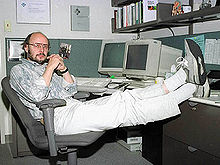
\includegraphics[height=3cm]{220px-BjarneStroustrup.jpg}
        %%\par{\usebeamercolor[fg]{caption name}%
            %%\usebeamerfont*{caption name}\figurename%
        %%\usebeamertemplate{caption label separator}}%
        %%\raggedright%
        %%\usebeamerfont*{caption}%
        %%Bjarne Stroustrup%
    %}

    %\opencutright

    %\begin{cutout}{0}{.65\linewidth}{0pt}{6}
    \begin{itemize}
        \item<1->Started by Bjarne Stroustrup in 1979 as "C with Classes"
            \begin{itemize}
                \item At Bell labs
                \item "Down the hall" from Dennis Ritchie (creator of C)
            \end{itemize}
        \item<1->Renamed to C++ in 1983, commercially implemented in 1985
        \item<2->1990s: stream IO, STL, ISO Standard in 98
        \item<3->2000s: Boost, TR1 in 2007
        \item<4->2010s: C++11 in 2011
    \end{itemize}
    %\end{cutout}
\end{frame}

\begin{frame}
    \frametitle{C Compilation model}

\end{frame}

\end{document}
